\documentclass[simplex.tex]{subfiles}
% NO NEED TO INPUT PREAMBLES HERE
% packages are inherited; you can compile this on its own
\providecommand{\mb}[1]{\boldsymbol{#1}}
\providecommand{\mv}[1]{\vec{#1}}
\providecommand{\ve}[1]{\boldsymbol{#1}}
\newcommand{\bpsi}{\ve{\psi}}
\newcommand{\bv}{\mb{v}}
\newcommand{\bx}{\mb{x}}
\newcommand{\bA}{\mathbf{A}}
\newcommand{\bH}{\mathbf{H}}
\newcommand{\bX}{\mathbf{X}}
\newcommand{\bP}{\mathbf{P}}
\newcommand{\bB}{\mathbf{B}}
\newcommand{\bD}{\mathbf{D}}
\newcommand{\bS}{\mathbf{S}}
\newcommand{\bR}{\mathbf{R}}
\newcommand{\bJ}{\mathbf{J}}
\newcommand{\bLambda}{\mathbf{\Lambda}}
\begin{document}
\subsection{Vertex Screening}
We are developing a vertex screening method to recover the signal subgraph. Specifically, we have $m$ pairs of graph and label sampled independently from some distribution $F_{G,Y}$,
\[(G_1,Y_1),(G_2,Y_2),(G_3,Y_3),...,(G_m,Y_m) \overset{i.i.d.}{\sim} F_{G,Y}. \] 
It is often the case that the signal is sparse in $G$. That is to say, there is a small subgraph $G[S]$ induced by signal vertices $S$ which contains all information about $Y$. The vertex screening method wants to recover the signal vertices $S$. It consists of three steps: feature extraction, computing distance correlations, and thresholding. \\

The first step is to extract a feature vector for each vertex in a graph. We use notation $\hat{X}_{i}[u,\cdot]$ to denote the feature extracted for vertex $u$ in graph $i$ where $i \in [m]$ and $u \in [n]$. A simple approach to obtain a feature vector is to set $\hat{X}_{i}[u]$ to the $u$th row of adjacency matrix $A_i$, that is $\hat{X}_{i}[u,\cdot]=A_i[u,\cdot]$. In this case,  $\hat{X}_{i}[u,\cdot]$ is a vector in $\mathbb{R}^n$ which can be a high dimensional space. Alternatively, Adjacency Spectral Embedding could also extract a feature vector $\hat{X}_{i}[u,\cdot]$ which lies in $\mathbb{R}^d$. The second step computes a correlation between  $\{\hat{X}_{i}[u,\cdot]\}_{i=1}^m$ and $\{Y_i\}_{i=1}^m$ for each $u \in V$. The correlation could be distance correlation (Dcorr) or multiscale generalized correlation (MGC). Let $c_u$ be the correlation, that is
\[ c_u = Dcorr(\{\hat{X}_{i}[u,\cdot]\}_{i=1}^m, \{Y_i\}_{i=1}^m ) \text{ or } MGC(\{\hat{X}_{i}[u,\cdot]\}_{i=1}^m, \{Y_i\}_{i=1}^m). \]
The last step order $c_u$s by their magnitudes. Then, we threshold the correlations by a critical value $c$. The vertices survive thresholding will be the estimated signal vertices $\hat{S}$, that is 
\[\hat{S} = \{u \in V | c_u > c\}.\]
The estimated signal subgraph and the corresponding adjacency matrix $G[\hat{S}]$ and $A[\hat{S}]$. The Algorithm \ref{alg:vs} describes the general procedure of vertex screening using adjacency vector as feature and MGC. A simulation experiment is shown in the Figure \ref{fig:vs} which demonstrates that the vertex screening can significantly improve the graph classification performance for various sample size. We are currently working on theories of vertex screening and finishing the first draft.
\clearpage
\begin{algorithm}
	\caption{Vertex Screening. Find the signal vertex estimate $\hat{S}$.}
	\label{alg:vs}
	\begin{algorithmic}[1]
		\Procedure{Input $\{(A_i,Y_i)\}_{i=1}^m$ and $c \in [0,1]$}{}
		\For{$u=1:n$ }
		\State $c_u = MGC(\{\hat{X}_{i}[u,\cdot]\}_{i=1}^m, \{Y_i\}_{i=1}^m )$
		\EndFor
		\State Output $\hat{S} = \{u| c_u > c\}$
		\EndProcedure
	\end{algorithmic}
\end{algorithm}


%%%  FIGURE BLOCK
\begin{figure}[!h]
	\begin{cframed}
		\centering
		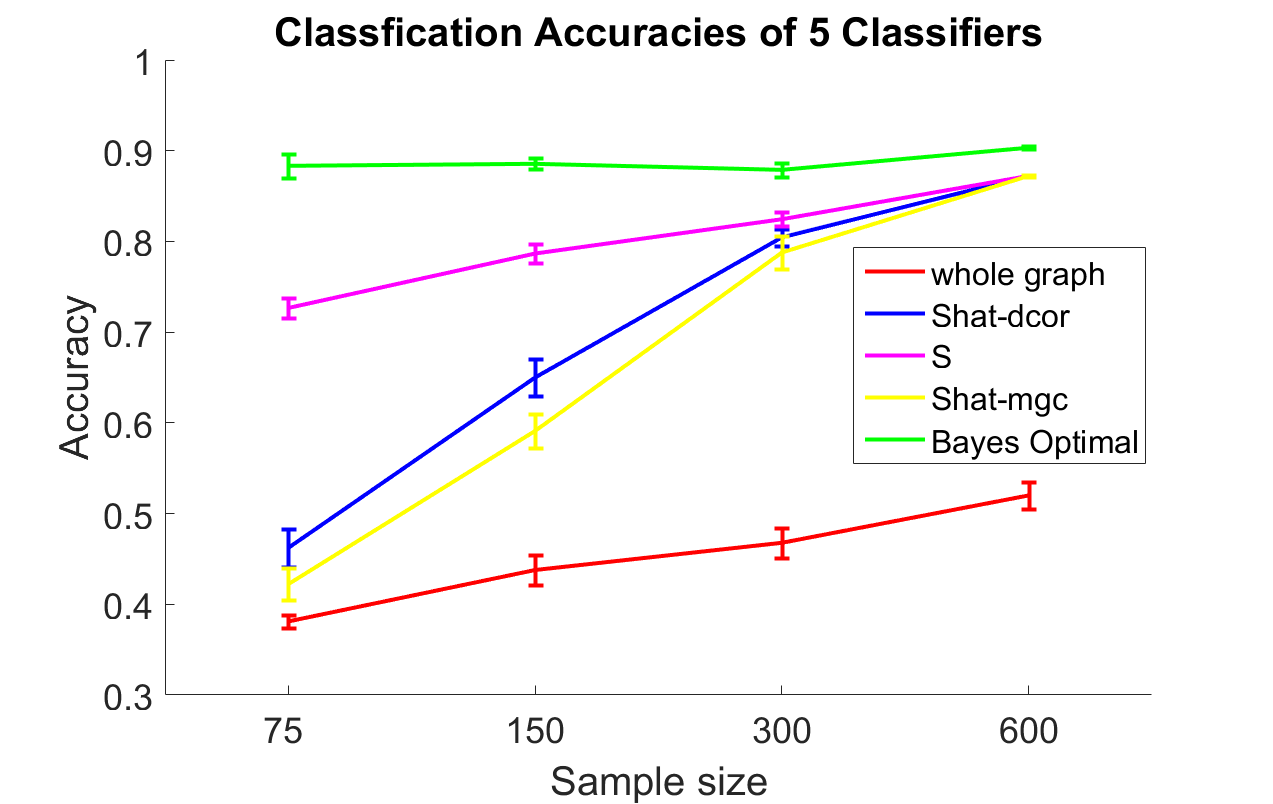
\includegraphics[scale=0.35, clip = true]{../../figs/Bayes_plugin_IER_3n.png}
		\caption{The classification accuracies of five approaches with their standard errors are shown. We generate graphs from $3$ different inhomogeneous Erdos-Renyi model, then apply $5$ classifiers to classify these graphs: Bayes optimal classifier (green), Bayes plugin on $G[S]$ (purple), Bayes plugin on $G[\hat{S}]$ with $\hat{S}$ estimated by Dcorr (blue), Bayes plugin on $G[\hat{S}]$ with $\hat{S}$ estimated by MGC (yellow), and Bayes plugin on $G$ (red). The classifiers with vertex screening (blue and yellow) have significantly better classification performance compared to without screening (red), and are close to Bayes optimal (green) when given $600$ graphs. }
		\label{fig:vs}
	\end{cframed}
\end{figure}
%
\clearpage

\subsection{Joint Embedding}
The latest draft is posted on \href{https://arxiv.org/abs/1703.03862}{arXiv} and submitted for publication. The code can be found \href{https://github.com/shangsiwang/Joint-Embedding}{here}. We are also working on making a R package with joint embedding included.



\clearpage

\end{document}
